\let\negmedspace\undefined
\let\negthickspace\undefined
\documentclass[journal]{IEEEtran}
\usepackage[a5paper, margin=10mm, onecolumn]{geometry}
%\usepackage{lmodern} % Ensure lmodern is loaded for pdflatex
\usepackage{tfrupee} % Include tfrupee package

\setlength{\headheight}{1cm} % Set the height of the header box
\setlength{\headsep}{0mm}  % Set the distance between the header box and the top of the text

\usepackage{gvv-book}
\usepackage{gvv}
\usepackage{cite}
\usepackage{amsmath,amssymb,amsfonts,amsthm}
\usepackage{algorithmic}
\usepackage{graphicx}
\usepackage{textcomp}
\usepackage{xcolor}
\usepackage{txfonts}
\usepackage{listings}
\usepackage{enumitem}
\usepackage{mathtools}
\usepackage{gensymb}
\usepackage{comment}
\usepackage[breaklinks=true]{hyperref}
\usepackage{tkz-euclide} 
\usepackage{listings}
% \usepackage{gvv}                                        
\def\inputGnumericTable{}                                 
\usepackage[latin1]{inputenc}                                
\usepackage{color}                                            
\usepackage{array}                                            
\usepackage{longtable}                                       
\usepackage{calc}                                             
\usepackage{multirow}                                         
\usepackage{hhline}                                           
\usepackage{ifthen}                                           
\usepackage{lscape}
\usepackage{tikz}
\usepackage{amsmath}
\usepackage{circuitikz}
\usepackage{tikz}
\usepackage{pgfplots}

\begin{document} 

\bibliographystyle{IEEEtran}
\vspace{3cm}

\title{2023-GATE-MA-1-13}
\author{EE24BTECH11029- JANAGANI SHRETHAN REDDY}
\maketitle{}
%\newpage
\bigskip
\renewcommand{\thefigure}{\theenumi}
\renewcommand{\thetable}{\theenum}
%section-1:carry one mark
\begin{enumerate}
    \item The village was nestled in a green spot,$\_\_\_$ the ocean and the hills.
    \begin{enumerate}
        \item through
        \item in
        \item at
        \item between
    \end{enumerate}
    \item Disagree : Protest :: Agree : $\_\_\_$
    \begin{enumerate}
        \item Refuse
        \item Pretext
        \item Recommend
        \item Refute
    \end{enumerate}
    \item A frabjous number is defined as a $3$ digit number with all digits odd, and no two adjacent digits being the same. For example, $137$ is a frabjous number, while $133$ is not. How many such frabjous numbers exist?
    \begin{enumerate}
        \item $125$
        \item $720$
        \item  $60$
        \item $80$
    \end{enumerate}
    \item Which one among the following statements must be TRUE about the mean and the median of the scores of all candidates for GATE $2023?$
    \begin{enumerate}
        \item The median is at least as large as the mean.
        \item The mean is at least as large as the median.
        \item At most half the candidates have a score that is lager than the median.
        \item At most half the candidates have a score that is lager than the mean.
    \end{enumerate}
    \item In the given diagram, ovals are marked at different heights $\brak{h}$ of a hill. Which one of the following options $P, Q, R, $and $S$ depicts the top view of the hill?

\begin{tikzpicture}
\begin{axis}[
    width=10cm, height=6cm,
    xlabel={Distance (in km)},
    ylabel={Height from mean sea level, $h$ (in km)},
    ymin=0, ymax=0.8,
    xmin=0, xmax=1.1,
    ytick={0, 0.2, 0.4, 0.6, 0.8},
    xtick={0, 0.2, 0.4, 0.6, 0.8, 1},
    axis lines=left,
    xlabel near ticks,
    ylabel near ticks,
]

% Draw hill shape
\addplot[black, thick, domain=0:1] {0.8*exp(-10*(x-0.25)^2)};

% Draw cross-sectional ellipses at different altitudes
\foreach \y in {0.1, 0.2, 0.3, 0.4, 0.5, 0.6, 0.7} {
    \addplot[blue, thick, samples=50, domain=0:1, variable=\t] 
    ({0.25 + 0.5 * \y * cos(deg(\t))}, {\y});
}

% Label for the hill
\node at (axis cs:0.45,0.75) {Hill};

% Draw the ellipse illustration in the legend area
\draw[blue, thick] (axis cs:0.8,0.5) ellipse [x radius=0.07, y radius=0.02];
\node[align=center] at (axis cs:0.8,0.4) {Horizontal cross-sections \\ at various altitudes ($h$)};
\end{axis}
\end{tikzpicture}\\
    \begin{enumerate}
        \item $P$
        \item $Q$
        \item $R$
        \item $S$
    \end{enumerate}
    \item Residency is a famous housing complex with many well-established individuals among its residents. A recent survey conducted among the residents of the complex revealed that all of those residents who are well established in their respective fields happen to be academicians. The survey also revealed that most of these academicians are authors of some best-selling books.\\
    Based only on the information provided above, which one of the following statements can be logically inferred with certainty?
    \begin{enumerate}
        \item Some residents of the complex who are well established in their fields are also authors of some best-selling books
        \item All academicians residing in the complex are well established in their fields
        \item Some authors of best-selling books are residents of the complex who are well established in their fields
        \item Some academicians residing in the complex are well established in their fields.
    \end{enumerate}
    \item Ankita has to climb $5$ stairs starting at ground, while respecting the following rules:\\
    $1.$ At any stage, Ankita can move either one or two stairs up.\\
    $2.$ At any stage, Ankita cannot move to a lower step.\\
    Let $F\brak{N}$ denote the number of possible ways in which Ankita can reach the $N^{th}$ stair.For example,$F\brak{1}=1,F\brak{2}=2,F\brak{3}=3.$\\
    The value of $F\brak{5}$ is
    \begin{enumerate}
        \item $8$
        \item $7$
        \item $6$
        \item $5$\\
    \end{enumerate}
   \item The information contained in DNA is used to synthesize proteins that are necessary for the functioning of life. DNA is composed of four nucleotides: Adenine ($A$), Thymine ($T$), Cytosine ($C$), and Guanine ($G$). The information contained in DNA can then be thought of as a sequence of these four nucleotides: $A$, $T$, $C$, and $G$. DNA has coding and non-coding regions. Coding regions—where the sequence of these nucleotides is read in groups of three to produce individual amino acids—constitute only about $2\%$ of human DNA. For example, the triplet of nucleotides CCG codes for the amino acid glycine, while the triplet GGA codes for the amino acid proline. Multiple amino acids are then assembled to form a protein.\\
    Based only on the information provided above, which of the following statements can be logically inferred with certainty?\\
    $\brak{i}$ The majority of human DNA has no role in the synthesis of proteins.\\
    $\brak{ii}$ The function of about $98\%$ of human DNA is not understood
    \begin{enumerate}
        \item Only $\brak{i}$
        \item Only $\brak{ii}$
        \item both $\brak{i}$ and $\brak{ii}$
        \item neither $\brak{i}$ nor $\brak{ii}$\\
    \end{enumerate}
    \item Which one of the figures $P,Q,R$ and $S$ represents the graph of the following function?\\
    $f\brak{x}=\abs{\abs{x+2}-\abs{x-1}}$
\begin{tikzpicture}
\begin{axis}[
    axis lines=middle,
    xmin=-5, xmax=5,
    ymin=0, ymax=4,
    xtick={-4, -2, 0, 2, 4},
    ytick={0, 1, 2, 3, 4},
    xlabel={$x$},
    ylabel={$f(x)$},
    ylabel style={rotate=-90},
    axis line style={gray},
    tick label style={font=\small},
]

% Draw the function
\addplot[
    blue, thick,
    domain=-4:4,
] coordinates {
    (-4,3) (-2,3) (-1,1) (1,1) (2,3) (4,3)
};

% Add label "P"
\node[anchor=south, font=\bfseries\Large] at (axis cs:0,3.2) {P};

\end{axis}
\end{tikzpicture}
    \begin{enumerate}
        \item $P$
        \item $Q$
        \item $R$
        \item $S$\\
    \end{enumerate}
    \item An opaque cylinder is suspended in the path of a parallel beam of light, such that its shadow is cast on a screen oriented perpendicular to the direction of the light beam. The cylinder can be reoriented in any direction within the light beam. Under these conditions, which one of the shadows $P, Q, R,$ and $S$ is NOT possible?\\
\begin{tikzpicture}

% Cylinder parameters
\def\height{3.5} % height of the cylinder
\def\radius{1} % radius of the cylinder

% Draw the main body of the cylinder
\fill[gray!20] (0,0) -- ++(0,\height) arc[start angle=180, end angle=360, x radius=\radius, y radius=0.5] -- ++(0,-\height) arc[start angle=0, end angle=180, x radius=\radius, y radius=0.5];

% Draw the outline of the cylinder
\draw (0,0) -- ++(0,\height);
\draw (2*\radius,0) -- ++(0,\height);
\draw (0,\height) arc[start angle=180, end angle=360, x radius=\radius, y radius=0.5];
\draw[dashed] (0,0) arc[start angle=180, end angle=0, x radius=\radius, y radius=0.5];

% Draw the top circle
\draw (0,\height) arc[start angle=180, end angle=0, x radius=\radius, y radius=0.5];
\end{tikzpicture}\\
\begin{tikzpicture}
    % Draw a circle with radius 2 units
    \draw (0,0) circle[radius=1.5];
    \node at (0,0) {P};
\end{tikzpicture}\\
\begin{tikzpicture}
    % Draw the rounded rectangle with a gray fill
    \fill[gray] (0,0) -- ++(2,0) arc[start angle=270, end angle=90, radius=1] -- ++(-2,0) arc[start angle=90, end angle=270, radius=1];
    
    % Add the text "Q" in the center
    \node at (0.5,0.75) {\textbf{Q}};
\end{tikzpicture}\\
\begin{tikzpicture}
    % Draw a rectangle with width 4 units and height 2 units
    \draw (0,0) rectangle (4,2);
    \node at (2,1) {R};
\end{tikzpicture}\\
\begin{tikzpicture}
    % Draw a square with side length 2 units
    \draw (0,0) rectangle (2,2);
    \node at (1,1) {s};
\end{tikzpicture}

    \begin{enumerate}
        \item $P$
        \item $Q$
        \item $R$
        \item $S$
    \end{enumerate}
    
    %carry one mark each
    \item Let $f,g\colon\mathbb{R}^2\rightarrow\mathbb{R}$ be defined by\\
    $f\brak{x,y}=x^2-\frac{3}{2}xy^2$ and $g\brak{x,y}=4x^4-5x^2y+y^2$\\
    for all $\brak{x,y}\in \mathbb{R}^2$\\
    Consider the following statements:\\
    $P\colon$ $f$ has a saddle point at $\brak{0,0}.$
    $Q\colon$ $g$ has a saddle point at $\brak{0,0}.$\\
    Then
    \begin{enumerate}
        \item both $p$ and $Q$ are true
        \item both $p$ and $Q$ are false
        \item $P$ is FALSE but $Q$ is TRUE
        \item $Q$ is FALSE but $P$ is TRUE
    \end{enumerate}
    \item Let $\mathbb{R}^3$ be a topological space with the usual topology and $\mathbb{Q}$ denote the set of rational numbers. Define the subspaces $X,Y,Z$ and $W$ of $\mathbb{R}^3$ as follows:
    $X=\cbrak{\brak{x,y,z}\in \mathbb{R}^3\colon \abs{x}+\abs{y}+\abs{z}\in\mathbb{Q}}
    \\Y=\cbrak{\brak{x,y,z}\in \mathbb{R}^3\colon xyz=1}\\
    Z=\cbrak{\brak{x,y,z}\in \mathbb{R}^3\colon x^2+y^2+z^2=1}\\
    W=\cbrak{\brak{x,y,z}\in \mathbb{R}^3\colon xyz=0}$\\
    Which of the following statements is correct?
    \begin{enumerate}
        \item $X$ is homeomorphic to $Y$
        \item $Z$ is homeomorphic to $W$
        \item $Y$ is homeomorphic to $W$
        \item $X$ is NOT homeomorphic to $W$
    \end{enumerate}
    \item Let $P\brak{x}=1+e^{2\pi ix}+2e^{3\pi ix},x\in \mathbb{R},i=\sqrt{-1}.$Then\\
    $\lim_{N\rightarrow\infty}\frac{1}{N}\sum_{k=0}^{N-1}P\brak{k\sqrt{2}}$\\
    is equal to
    \begin{enumerate}
        \item $0$
        \item $1$
        \item $3$
        \item $4$
    \end{enumerate}
\end{enumerate}
\end{document}
